\documentclass[a4paper,11pt,notitlepage,fullpage]{article}
%\documentclass{report}

\usepackage{fullpage}
\usepackage[utf8]{inputenc}
\usepackage[ngerman]{babel}
%\usepackage[english]{babel}
\usepackage{amsmath}
\usepackage{amssymb}
\usepackage{latexsym}
\usepackage{mathtools}
\usepackage{listings}
\usepackage{bbm}
%\usepackage{algorithm}
%\usepackage{algpseudocode}
\usepackage{graphicx}
\usepackage{booktabs}
\usepackage{hhline}
\usepackage{amsthm}
\usepackage{cite}
\usepackage{wrapfig}
\usepackage{hyperref}
\usepackage{titling}
\usepackage{color}

\setlength{\droptitle}{-60pt}

\newcommand{\R}{\mathbb R}
\newcommand{\p}{\mathbb P}
\newcommand{\pp}[1]{\mathbb P\left[#1\right]}
\newcommand{\E}{\mathbb E}
\newcommand{\Ee}[1]{\mathbb E\left[#1\right]}
\newcommand{\V}{\mathbb V}
\newcommand{\Vv}[1]{\mathbb V\left[#1\right]}
\newcommand{\Cov}[1]{\mathbb Cov\left[#1\right]}
\newcommand{\F}{\mathcal{F}}
\newcommand{\ind}{\mathbbm{1}}
\newcommand{\indd}[1]{\mathbbm{1}_{#1}}
\newcommand{\norm}[2]{\left|\left|{#1}\right|\right|_{#2}}

\begin{document}
\author{Florian Bogner \& Alexander Palmrich}
\title{Stochastische Prozesse - Übung 6}
\maketitle

\begin{enumerate}
\setcounter{enumi}{24}

%%für ein Bild das copy-pasten und reinkommentieren
%\begin{figure}[h!]
%\centering
%\includegraphics[width=0.9\textwidth]{gfx/bildname.png}
%\label{fig1}
%\caption{TODO Beschreibung des Bildes}
%\end{figure}

%01
\item $f(t):=e^{\alpha t}$
\begin{enumerate}
%a
\item $f\in M^2$? $f\in M^2_T$? Für welche $\alpha$ jeweils?

$f$ ist deterministisch, somit adaptiert, und hat stetige Pfade. Laut VO ist es hinreichend dass die Norm endlich ist um in den jeweiligen Räumen zu liegen. Wenn die Norm unendlich groß ist, ist $f$ nicht im jeweiligen Raum laut Defintion. Also gilt für jedes $\alpha$ einzeln $f\in M^2_T \Leftrightarrow \norm{f}{M^2_T}<\infty$ und $f\in M^2 \Leftrightarrow \norm{f}{M^2}<\infty$.
\begin{align*}
\norm{f}{M^2_T} &= \Ee{\int_0^T (e^{\alpha t})^2 dt}\\
&= \Ee{\int_0^T e^{2\alpha t} dt}\\
&= \Ee{\left[\frac{e^{2\alpha t}}{2\alpha}\right]_{t=0}^{t=T}}\\
&= \Ee{\frac{e^{2\alpha T}-1}{2\alpha}}\\
&= \frac{e^{2\alpha T}-1}{2\alpha} < \infty \text{ für alle } \alpha \in \mathbb{R}^*
\end{align*}
Für $\alpha=0$ versagt obige Darstellung, wir müssen diesen Fall extra behandeln: Da integrieren wir $f=1$ konstant über ein Kompaktum, das bleibt beschränkt.

Wenn wir statt bis $T$ über ganz $\mathbb{R}^+$ integrieren, dann ist das Integral unbeschränkt für alle $\alpha\geq 0$ und endlich sonst. ($\sim$ Dichte einer Exponentialverteilung!)

%b
\item $I_T(f):= \int_0^T f(t) dW(t)$, davon $\E$ und $\V$ berechnen für $\alpha=\ln 2, T=\sqrt{13}$.

Wegen Martingaleigenschaft ist $\Ee{I_T(f)} = 0$.
\begin{align*}
\Vv{I_T(f)} &= \Ee{(I_T(f))^2} - 0^2\\
&=\Ee{\int_0^T f^2 dt} &\text{Itô-Iso}\\
&=\Ee{\int_0^T e^{2\alpha t} dt}\\
&= \frac{e^{2\alpha T}-1}{2\alpha}\\
&= \frac{e^{2\ln 2 \sqrt{13}}-1}{2\ln 2}\\
&= \frac{2^{2\sqrt{13}}-1}{2\ln 2}
\end{align*}

%c
\item $g(t,x):= t^3e^{-x}, Y(t):=g(t, W(t))$ in Differentialschreibweise der Itô-Formel angeben.
\begin{align*}
g_t &= 3t^2e^{-x}\\
g_x &= -3t^3e^{-x}\\
g_{xx} &= 3t^3e^{-x} = g\\
\end{align*}
Integraldarstellung:
\begin{align*}
Y(T) &= g(t, W(t))\\
&= g(0, W(0)) + \int_0^T g_x(t, W(t)) dW(t) + \int_0^T g_t(t, W(t)) + \frac{1}{2} g_{xx}(t, W(t)) dt\\
\end{align*}
in Differentialdarstellung:
\begin{align*}
dg &= g_x + g_t + \frac{1}{2} g_{xx}\\
&= -3t^3e^{-x} + 3t^2e^{-x} + \frac{1}{2} 3t^3e^{-x}\\
&= 3t^2e^{-x} \left(-t +1 +\frac{t}{2} \right)\\
&= \left(\frac{1}{t} -\frac{1}{2} \right)g
\end{align*}

\end{enumerate}

%02
\item bla
\begin{enumerate}
%a
\item a
\begin{align*}
\end{align*}

%b
\item b
\begin{align*}
\end{align*}
\end{enumerate}

%03
\item Wir nummerieren die Räume von 1 bis 6 zeilenweise, i.e. der Start ist 1, der Käse ist 5 und die Falle ist 6. Die Anfangsverteilung lautet $\lambda = (1,0,0,0,0,0)$ und die Übergangsmatrix lautet dann
$$P = \begin{pmatrix}
&\frac{1}{2}&\frac{1}{2}&&& \\
\frac{1}{2}&&&\frac{1}{2}&& \\
\frac{1}{3}&&&\frac{1}{3}&\frac{1}{3}& \\
&\frac{1}{3}&\frac{1}{3}&&&\frac{1}{3} \\
&&&&1& \\
&&&&&1 
\end{pmatrix}$$
In der Sprache der Markovketten sind Zustände 5 und 6 absorbierend. Die anderen Zustände sind transient. Wir suchen die Absorbtionswahrscheinlichkeit des Zustands 6 unter der gegebenen Anfangsverteilung.
Sei $p_i$ die Absorbtionswahrscheinlichkeit des Zustands 6, wenn man in Zustand $i$ startet. Offensichtlich gilt $p_5 = 0$ und $p_6 = 1$. Die anderen $p_i$ erfüllen ein Gleichungsystem. Die Absorbtionswahrscheinlichkeit ist der nach Übergangswahrscheinlichkeiten gewichtete Durchschnitt der anderen Absorbtionswahrscheinlichkeiten.
$$p_i = \sum_j P_{ij} p_j$$
Außerdem, aufgrund der Symmetrie in dem Irrgarten gilt $p_1 = 1 - p_2$ und $p_3 = 1-p_4$. Zusammengefasst und eingesetzt bekommt man die zwei Gleichungen:
\begin{align*}
p_1 &= \frac{1}{2}(1 - p_1 + p_3) \\
p_3 &= \frac{1}{3}(p_1 + 1 - p_3 + 0)
\end{align*}
Umgeformt:
\begin{align*}
3 p_1 - 1&= p_3 \\
- p_1 + 4 p_3 &= 1
\end{align*}
Erste Gleichung in zweite eingesetzt ergibt:
$$- p_1 + 4 (3 p_1 - 1) = 1$$
$$11 p_1 - 4 = 1$$
$$p_1 = \frac{5}{11}$$
Wir müssen $p_3$ gar nicht mehr berechnen, da $p_1$ gleich unsere Antwort ist: Die Maus tappt mit Wahrscheinlichtkeit $\frac{5}{11}$ in die Falle. Armes Mausi.

%04
\item Mit dem Satz der Totalen Wahrscheinlichkeit und der Eigenschaft strikt stationär geht das ganz ez:
\begin{align*}
\lambda_0 &= \pp{X_0 = 0} \\
&= \pp{X_0 = 0, X_1 = 0} + \pp{X_0 = 0, X_1 = 1} \\
&= 0.25+0.15 = 0.4 \\
\lambda_1 &= 1-\lambda_0 = 0.6 \\
P_{00} &= \pp{X_{n+1} = 0 | X_n = 0} \\
&= \pp{X_{n+1} = 0 | X_n = 0, X_{n-1} = 0}\cdot\pp{X_{n-1} = 0} + \cdots \\
&~~~~\cdots + \pp{X_{n+1} = 0 | X_n = 0, X_{n-1} = 1}\cdot\pp{X_{n-1} = 1} \\
&= 0.7 \cdot \lambda_0 + 0.5 \cdot \lambda_1 \\
&= 0.58 \\
P_{10} &= \pp{X_{n+1} = 0 | X_n = 1} \\
&= \pp{X_{n+1} = 1 | X_n = 1, X_{n-1} = 0}\cdot\pp{X_{n-1} = 0} + \cdots \\
&~~~~\cdots + \pp{X_{n+1} = 0 | X_n = 1, X_{n-1} = 1}\cdot\pp{X_{n-1} = 1} \\
&= 0.4 \cdot \lambda_0 + 0.2 \cdot \lambda_1 \\
&= 0.28 \\
P_{01} &= 1 - P_{00} = 0.42 \\
P_{11} &= 1 - P_{10} = 0.72
\end{align*}
TODO: Überlegen ob das richtig ist. Kann man aus der strikt stationär Eigenschaft wirklich schließen, dass die unbedingte Verteilung die gleiche ist wie die Startverteilung? Außerdem muss man eigentlich zeigen, dass X strikt stationär ist.

Laut Markov-Eigenschaft müsste dann ja z.B. $$\pp{X_{n+1} = 0 | X_n = 0} = \pp{X_{n+1} = 0 | X_n = 0, X_{n-1} = 0}$$ gelten, aber klarerweise ist $0.58 \neq 0.7$.

Wir definieren uns eine Markovkette: Als Zustandsraum $S := \{00, 10, 01, 11\}$ wählen wir Zusammenfassungen von je zwei Tagen. Die Anfangsverteilung $\lambda := (0.25, 0.15, 0.15, 0.45)$ lesen wir direkt aus der Tabelle ab. Die Berechnung der Übergangswahrscheinlichkeiten ist einen Hauch komplizierter. Sei $a, b, c, d \in \{0, 1\}$
\begin{align*}
P_{ab, cd} &= \pp{X_{n+2} = d, X_{n+1} = c | X_n = b, X_{n-1} = a} \\
&= \pp{X_{n+1} = c | X_n = b, X_{n-1} = a} \cdot \pp{X_{n+2} = d | X_{n+1} = c, X_n = b, X_{n-1} = a} \\
&= \pp{X_{n+1} = c | X_n = b, X_{n-1} = a} \cdot \pp{X_{n+2} = d | X_{n+1} = c, X_n = b}
\end{align*}
Die vorkommenden Wahrscheinlichkeiten sind in der Tabelle zu finden. Wir wir rechenen illustrativ $P_{01,10}$ aus:
\begin{align*}
P_{01, 10} &= (1-0.4) \cdot 0.2 = 0.12
\end{align*}

%05
\item
\begin{figure}[h!]
\centering
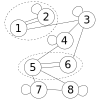
\includegraphics[width=0.5\textwidth]{gfx/29_a.pdf}
\caption{\label{fig:graph} Graph der Markovkette in 29 (a)}
\end{figure}

\begin{enumerate}
%a
\item Die Matrix lesbar aufgeschrieben lautet
\begin{align*}
P = \frac{1}{10}\begin{pmatrix}
&1&9&&&&&\\
1&9&&&&&&\\
&&6&2&&2&&\\
&&&5&5&&&\\
&&&&&4&3&3\\
&&&&10&&&\\
&&&&&&9&1\\
&&&&&&&10
\end{pmatrix}
\end{align*}
In Abbildung \ref{fig:graph} sehen wir eine graphische Representation der Markovkette. Nur positive Übergangswahrscheinlichkeiten sind eingezeichnet. Die einzige nichttriviale Kommunikationsklasse $\{1, 2\}$ ist strichliert eingezeichnet. Alle anderen Kommunikationsklassen enthalten nur einen Zustand. Damit ist die Markovkette reduzibel.
%b
%copypasta : P = np.array([[int(d) for d in line] for line in "0110 1001 0011 0011".split(" ")])/2
\item Behauptung für $n \geq 1$:
\begin{align*}
n~\text{gerade} &\Rightarrow P^n = \begin{pmatrix}
\frac{1}{2}^n&0&\frac{1}{2}-\frac{1}{2}^n&\frac{1}{2} \\
0&\frac{1}{2}^n&\frac{1}{2}&\frac{1}{2}-\frac{1}{2}^n \\
0&0&\frac{1}{2}&\frac{1}{2}\\
0&0&\frac{1}{2}&\frac{1}{2}
\end{pmatrix} \\
n~\text{ungerade} &\Rightarrow P^n = \begin{pmatrix}
0&\frac{1}{2}^n&\frac{1}{2}&\frac{1}{2}-\frac{1}{2}^n \\
\frac{1}{2}^n&0&\frac{1}{2}-\frac{1}{2}^n&\frac{1}{2} \\
0&0&\frac{1}{2}&\frac{1}{2}\\
0&0&\frac{1}{2}&\frac{1}{2}
\end{pmatrix} 
\end{align*}

Beweis per Induktion: Induktionsanfang \emph{trivial}.

Gerader Induktionsschritt:
\begin{gather*}
P^n = P^{n-1} \cdot P = \begin{pmatrix}
0&\frac{1}{2}^{n-1}&\frac{1}{2}&\frac{1}{2}-\frac{1}{2}^{n-1} \\
\frac{1}{2}^{n-1}&0&\frac{1}{2}-\frac{1}{2}^{n-1}&\frac{1}{2} \\
0&0&\frac{1}{2}&\frac{1}{2}\\
0&0&\frac{1}{2}&\frac{1}{2}
\end{pmatrix} \cdot \begin{pmatrix}
0&\frac{1}{2}&\frac{1}{2}&0 \\
\frac{1}{2}&0&0&\frac{1}{2} \\
0&0&\frac{1}{2}&\frac{1}{2}\\
0&0&\frac{1}{2}&\frac{1}{2}
\end{pmatrix} \\
= \begin{pmatrix}
\frac{1}{2}^{n-1} \cdot \frac{1}{2} & 0 & \frac{1}{2}\cdot\frac{1}{2} + (\frac{1}{2} - \frac{1}{2}^{n-1})\cdot\frac{1}{2} & \frac{1}{2}^{n-1} \cdot \frac{1}{2} + \frac{1}{2}\cdot\frac{1}{2} +  (\frac{1}{2} - \frac{1}{2}^{n-1})\cdot\frac{1}{2}\\
0 & \frac{1}{2}^{n-1} \cdot \frac{1}{2} & \frac{1}{2}^{n-1} \cdot \frac{1}{2} + \frac{1}{2}\cdot\frac{1}{2} +  (\frac{1}{2} - \frac{1}{2}^{n-1})\cdot\frac{1}{2} & \frac{1}{2}\cdot\frac{1}{2} + (\frac{1}{2} - \frac{1}{2}^{n-1})\cdot\frac{1}{2} \\
0&0&\frac{1}{2}\cdot\frac{1}{2} + \frac{1}{2}\cdot\frac{1}{2}&\frac{1}{2}\cdot\frac{1}{2} + \frac{1}{2}\cdot\frac{1}{2}\\
0&0&\frac{1}{2}\cdot\frac{1}{2} + \frac{1}{2}\cdot\frac{1}{2}&\frac{1}{2}\cdot\frac{1}{2} + \frac{1}{2}\cdot\frac{1}{2}
\end{pmatrix} \\
= \begin{pmatrix}
\frac{1}{2}^n&0&\frac{1}{2}-\frac{1}{2}^n&\frac{1}{2} \\
0&\frac{1}{2}^n&\frac{1}{2}&\frac{1}{2}-\frac{1}{2}^n \\
0&0&\frac{1}{2}&\frac{1}{2}\\
0&0&\frac{1}{2}&\frac{1}{2}
\end{pmatrix}
\end{gather*}

Ungerader Induktionsschritt analog:
\begin{gather*}
P^n = P^{n-1} \cdot P = \begin{pmatrix}
\frac{1}{2}^{n-1}&0&\frac{1}{2}-\frac{1}{2}^{n-1}&\frac{1}{2} \\
0&\frac{1}{2}^{n-1}&\frac{1}{2}&\frac{1}{2}-\frac{1}{2}^{n-1} \\
0&0&\frac{1}{2}&\frac{1}{2}\\
0&0&\frac{1}{2}&\frac{1}{2}
\end{pmatrix} \cdot \begin{pmatrix}
0&\frac{1}{2}&\frac{1}{2}&0 \\
\frac{1}{2}&0&0&\frac{1}{2} \\
0&0&\frac{1}{2}&\frac{1}{2}\\
0&0&\frac{1}{2}&\frac{1}{2}
\end{pmatrix} \\
= \begin{pmatrix}
0 & \frac{1}{2}^{n-1} \cdot \frac{1}{2} & \frac{1}{2}^{n-1} \cdot \frac{1}{2} + \frac{1}{2}\cdot\frac{1}{2} +  (\frac{1}{2} - \frac{1}{2}^{n-1})\cdot\frac{1}{2} & \frac{1}{2}\cdot\frac{1}{2} + (\frac{1}{2} - \frac{1}{2}^{n-1})\cdot\frac{1}{2} \\
\frac{1}{2}^{n-1} \cdot \frac{1}{2} & 0 & \frac{1}{2}\cdot\frac{1}{2} + (\frac{1}{2} - \frac{1}{2}^{n-1})\cdot\frac{1}{2} & \frac{1}{2}^{n-1} \cdot \frac{1}{2} + \frac{1}{2}\cdot\frac{1}{2} +  (\frac{1}{2} - \frac{1}{2}^{n-1})\cdot\frac{1}{2}\\
0&0&\frac{1}{2}\cdot\frac{1}{2} + \frac{1}{2}\cdot\frac{1}{2}&\frac{1}{2}\cdot\frac{1}{2} + \frac{1}{2}\cdot\frac{1}{2}\\
0&0&\frac{1}{2}\cdot\frac{1}{2} + \frac{1}{2}\cdot\frac{1}{2}&\frac{1}{2}\cdot\frac{1}{2} + \frac{1}{2}\cdot\frac{1}{2}
\end{pmatrix} \\
= \begin{pmatrix}
0&\frac{1}{2}^n&\frac{1}{2}&\frac{1}{2}-\frac{1}{2}^n \\
\frac{1}{2}^n&0&\frac{1}{2}-\frac{1}{2}^n&\frac{1}{2} \\
0&0&\frac{1}{2}&\frac{1}{2}\\
0&0&\frac{1}{2}&\frac{1}{2}
\end{pmatrix}
\end{gather*}
\qed

Im Grenzwert:
\begin{align*}
P^\infty = \begin{pmatrix}
0&0&\frac{1}{2}&\frac{1}{2}\\
0&0&\frac{1}{2}&\frac{1}{2}\\
0&0&\frac{1}{2}&\frac{1}{2}\\
0&0&\frac{1}{2}&\frac{1}{2}
\end{pmatrix}
\end{align*}

Daraus sieht man die Zustände 1 und 2 sind gemeinsam in einer Kommunikationsklasse transient und analog sind die Zustände 3 und 4 in einer Kommunikationsklasse rekurrent.
\end{enumerate}

\end{enumerate}



\end{document}
